
\section{Gamedesign}\label{sec:Gamedesign}

\renewcommand{\kapitelautor}{Autor: Philip Jankovic}


\subsection{Problem des Revolverhandlings}\label{subsec:gamedesignBehindBullets}

Das wichtigste Ziel bei der Entwicklung von \FF war es, das der Spieler den Revolver richtig benützt. Damit ist gemeint,
den Spieler dazu zu bringen, jegliche Mechaniken des Revolvers zu nutzen und kreative Möglichkeiten zu finden, ihn optimal zu verwenden.
Das Erreichen des Ziels stellte sich zunächst als schwierig heraus, denn folgende Problematik tritt auf.


Der Spieler zieht ganz normal seine Karten und platziert eine Bullet im vordersten Slot des Revolvers.
Anstatt sich einen Revolver mit mehreren Bullets aufzubauen, platziert er die Bullet und schießt sie sofort ab.
Das Gleiche passiert mit der nächsten Bullet. Diese Art von Gameplay ist genau das, was vermieden werden sollte.
Es ist langweilig, unkreativ und fordert keinerlei Denkanstrengungen oder Gedanken des Spielers.


Dieses Problem hatte auch eine frühere Version von \FF. Um dieses Problem zu beheben, wurde ein Designprinzip
ins Leben gerufen, welches sich \quoted{Placement Matters} nennt.


\subsection{Placement matters}\label{subsec:placementMatters}

Placement Matters ist ein Begriff, der das Gamedesign von \FF gut beschreibt. Durch den Revolver, seine limitierenden
Eigenschaften und den begrenzten Platz entsteht durch diese Designphilosophie die erwünschte Spielweise der Spieler.

Placement Matters beschreibt das Konzept, dass beim Platzieren einer Kugel der Ort, die Reihenfolge und der Zeitpunkt
eine wichtige Rolle spielen. Durch Trigger wie zum Beispiel \quoted{On-Rotate} oder \quoted{On-Turn-Begin} profitieren manche Bullets davon,
am Ende des Revolvers platziert zu werden, damit sie trotz der Rotation so lange wie möglich im Revolver bleiben können.


Der Statuseffekt \quoted{Burning} zum Beispiel, erhöht den Schaden der nächsten paar Bullets um 50\%.
Durch diesen Effekt ist es also ratsam, Bullets mit diesem Effekt vor anderen Bullets abzufeuern, um mehr Schaden zu erzielen.


Durch \quoted{Leaders Bullet} werden alle Bullets gestärkt, solange sich \quoted{Leaders Bullets} im Revolver befindet. Platziert der Spieler sie also
weiter vorne im Revolver, verlieren alle Bullets den positiven Effekt, da \quoted{Leaders Bullet} vor ihnen den Revolver verlässt.


Der Effekt von \quoted{Guarding Angles Bullet} wiederum bezieht sich zum Beispiel auf einen bestimmten Slot, nämlich Slot 3,
was den Spieler dazu bringt, die Platzierung seiner Karten genau zu überdenken. Diese Einschränkungen und Herausforderungen
sind der Grundstein für das Revolver-Gameplay von \FF.


Trotz dieser Einschränkungen ist es wichtig, dem Spieler auch gewisse Freiheiten zu überlassen. Placement Matters darf
also nicht übertrieben werden, da der Spieler vor lauter Einschränkungen und Regeln, wie was zu platzieren ist, den Spaß
verliert und außerdem seinen eigenen Spielstil nicht entwickeln kann, wenn der einzig richtige Zug mit einer Karte bereits vordefiniert ist.



\subsection{Archetypedesign und Effektdesign}\label{subsec:placementMatters}

\FF's Karten können grob in Archetypen aufgeteilt werden. Ein Archetyp in Kartenspielen beschreibt eine bestimmte Strategie, welche Karten verfolgen.
Spieler können dann basierend auf diesen Archetypen Decks bauen und damit verschiedene Strategien verfolgen.\zit{whatIsAnArchetype}


In \FF wurde versucht, die Archetypen so breit wie möglich zu gestalten. Das bedeutet, dass es bereits dezidierte Archetypen gibt,
jedoch viele Karten in mehreren Archetypen spielbar sind und die Archetypen sich auch überschneiden.
Während der Entwicklung wurde dieses Konzept als \quoted{Broad Archetypes} bezeichnet. Gründe für diesen Ansatz sind unter anderem
die sehr speziellen Spielregeln von \FF und die zufällige Reihenfolge, in der der Spieler die Karten erhält.


Im Vergleich zu \quoted{Magic the Gathering}, wo die Archetypen strenger sind und sogar durch Farben voneinander getrennt werden,
kann sich der Spieler bei \FF nicht direkt aussuchen, welche Karten er gerne hätte, sondern muss eine von den drei Karten nehmen,
die ihm zufällig vorgelegt werden. Die regeln von \quoted{Magic the Gathering} sind außerdem viel breiter gefächert und basieren nicht auf einem limitierten
Konzept wie dem Revolver. \zit{magicarena}


Wenn ein Effekt einer Bullet also \quoted{On-Rotate} auslöst, ist er in vielen Decks spielbar und nicht nur in Decks
eines Rotation-Archetyps, da die Drehung des Revolvers häufig passiert.

Die in \FF verwendete Methode der Borad-Archetypes erlaubt dem Spieler unzählige Kombinationen und ermöglicht
in der Regel ein gutes Spielerlebniss beim Endecken neuer Kombination.


Ein gutes Beispiel für diese breiten Archetypen und die Interkonnektivität der Archetypen ist zum Beispiel \quoted{High Velocity Bullet}.
\quoted{High Velocity Bullet} ist eine ein Kosten, null Schaden Karte, die über den Effekt verfügt, dass sie dem Gegner Schaden zufügt, wenn sie \quoted{On-Leave} ist.
Für viele Spieler scheint diese Bullet jedoch bizarr. Der \quoted{On-Leave} Trigger ist bei \quoted{High Velocity Bullet} dafür verantwortlich,
dass wenn die Karte geschossen wird, der Gegner Schaden bekommt, obwohl \quoted{High Velocity Bullet} eine null bei ihrem Schadens-Wert hat.
Die Formulierung des Triggers erlaubt es, dass der Effekt von \quoted{High Velocity Bullet} durch jegliche Art und Weise, durch
die die Bullet den Revolver verlässt, aktiviert wird. Wenn der Spieler \quoted{High Velocity Bullet} das erste Mal verwendet,
ist sie nicht viel anders als eine normale Bullet, jedoch stößt der Spieler mit der Zeit auf \quoted{Deputies Bullet}.

\begin{figure}[H]
    \centering
    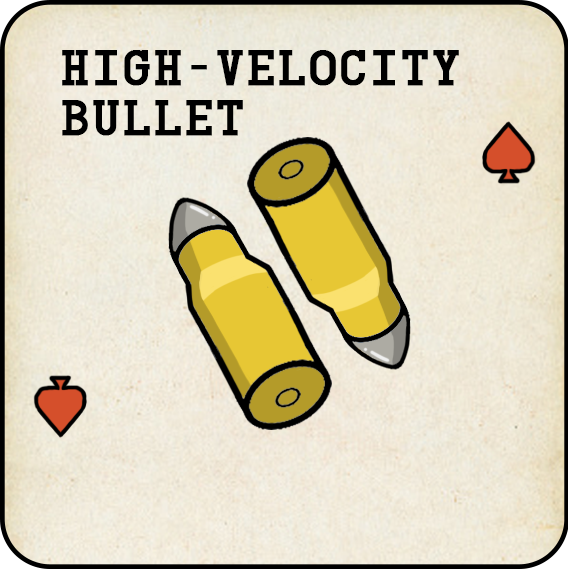
\includegraphics[width=0.5\textwidth]{highVB.png}
    \caption{Beispiel: \quoted{High Velocity Bullet}}
\end{figure}


\quoted{Deputies Bullet} hat den Effekt, dass wenn sie im Revolver platziert wird, die Karte welche sich im Slot 3 befindet wieder in die Hand
zurückgegeben wird. Auch hier kommt das bereits erwähnte Placement Matters ins Spiel, da der Spieler sich bewusst sein
muss, welche Karte auf seine Hand zurückgegeben wird, bevor er \quoted{Deputies Bullet} spielt. Zuerst wird der Spieler den
Effekt von \quoted{Deputies Bullet} als etwas Negatives sehen, um den erhöhten Schaden der Bullet auszugleichen,
eine bewusste Entscheidung, die später noch einmal ins Spiel kommt.

\begin{figure}[H]
    \centering
    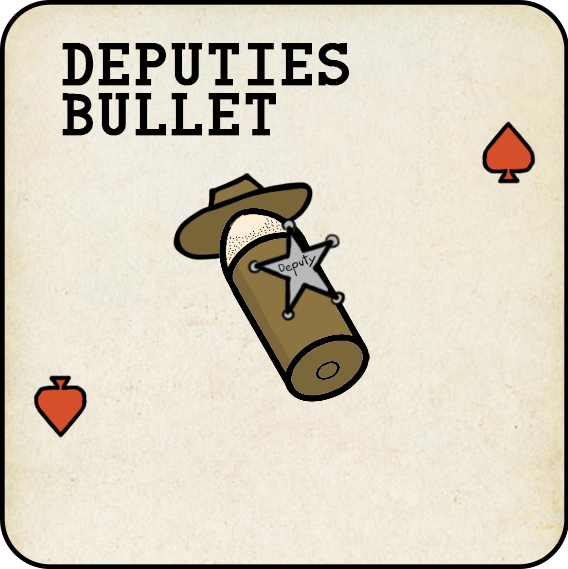
\includegraphics[width=0.5\textwidth]{deputiesB.png}
    \caption{Beispiel: \quoted{Deputies Bullet}}
\end{figure}

Kombiniert mit \quoted{High Velocity Bullet}, kann der eher negative Effekt von \quoted{Deputies Bullet} verwendet werden, um
\quoted{High Velocity Bullet} den Revolver verlassen zu lassen und damit vorzeitig dem Gegner Schaden zuzufügen.
Zusätzlich dazu, dass der Effekt von “Deputies Bullet”, umgangssprachlich \quoted{Bounce} genannt, \quoted{On-Leave} Effekte triggert,
ist es eine Möglichkeit Karten mit einem \quoted{On-Placedown} Trigger auf die Hand zu geben. Das erlaubt es, den Effekt damit noch einmal zu aktivieren.
Eine andere Möglichkeit ist, dass der Spieler auf eine \quoted{Purge Bullet} stößt. \quoted{Purge Bullet} hat ähnlich wie \quoted{Deputies Bullet}
erhöhten Schaden, dafür ist ihr Effekt, die Zerstörung von zwei Bullets neben ihr, wenn sie platziert wird.
Dies kann jedoch vom Spieler vermieden werden indem er - wieder durch Placement Matters- \quoted{Purge Bullet} auf eine Art und
Weise in den Revolver platziert, sodass keine Karte neben ihr liegt und damit auch nicht zerstört wird.
Ähnlich wie bei \quoted{Deputies Bullet} jedoch, kann \quoted{High Velocity Bullet} mit \quoted{Purge Bullet} zerstört werden, was wiederum als
Verlassen des Revolvers zählt, also den Effekt von \quoted{High Velocities} Bullet aktiviert. \quoted{Purge Bullet} ist außerdem Teil
des Destroy Archetypes, welcher darauf abzielt, dass Karten im Revolver zerstört werden.
Dieser relativ abgesonderte Archetype, kann trotzdem mit \quoted{On-Leave} Effekten kombiniert werden, was wiederum das breite
Kartendesign von \FF veranschaulicht.

\begin{figure}[H]
    \centering
    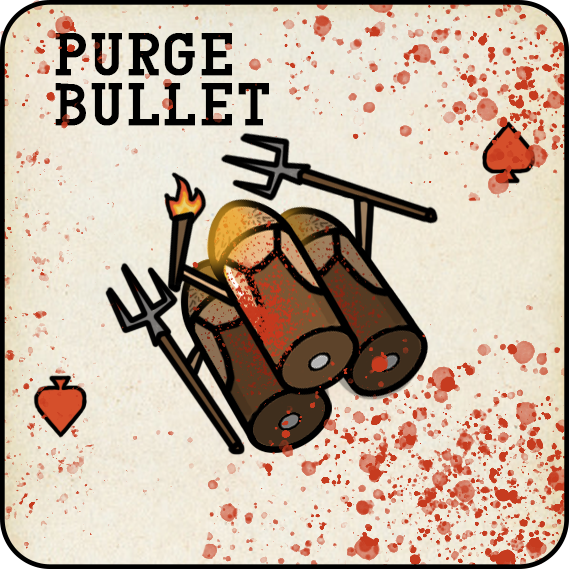
\includegraphics[width=0.5\textwidth]{purgeB.png}
    \caption{Beispiel: \quoted{Purge Bullet}}
\end{figure}


Der breite Ansatz ermöglicht es dem Spieler, mit fast jeder neuen Karte, die er erhält, neue Kombinationen und Nutzungsmöglichkeiten zu entdecken.
Es stärkt außerdem das Verständnis der Spielmechaniken.
Jedoch funktionieren nicht alle \FF Archetypen mit jedem anderen, es würde sonst den Spaß aus dem Deckbau nehmen.
Wäre das nämlich der Fall, wäre das Bauen eines Decks komplett obsolet und der Spieler müsste sich keine Gedanken darüber machen, wie er sein Deck zusammenstellt.



\subsection{Kartensammeln und Kartenpools}\label{subsec:placementMatters}

Durch die Vielzahl an Karten und den Unterschieden in der Komplexität zwischen diesen Karten werden Karten in \FF in \quoted{Pools} eingeteilt.
Diese Kartenpools dienen der Kontrolle, wann welche Karten vom Spieler nutzbar sind.
Sie halten komplexe und zu starke Karten vom Spieler fern, bis dieser bereit ist, sie zu erhalten.
Zum jetzigen Zeitpunkt gibt es zwei Kartenpools mit jeweils rund 25 Karten. Combos in Pool eins sind oft einfachere
Versionen der komplizierteren Combos, die durch Pool zwei Karten möglich sind.
Pool eins ist darauf ausgelegt, dass die Grundmechaniken von \FF dem Spieler bewusst werden.
%pool, draft usw


\subsection{Backback und Deck Gamedesign}\label{subsec:placementMatters}

Am Anfang des Spiels besitzt der Spieler sieben bis acht Bullets. Im Laufe des Spiels, sei es durch absolvierte Kämpfe
oder Map-Events, sammelt der Spieler Bullets. Wenn eine Bullet gesammelt wird, kann der Spieler sich entscheiden,
ob er die Karte in sein Deck gibt oder in den Rucksack. Hat er jedoch die Mindestanzahl an Bullets in seinem Deck
noch nicht erreicht, steht ihm nur das Hinzufügen zum Deck offen. Erst wenn der Spieler genug Bullets gesammelt hat,
um die Mindestanzahl des Decks einzuhalten, kann er Bullets aus dem Deck verschieben.


Es gibt einige Faktoren in \FF, die das Bauen bzw. die Wahl des Decks beeinflussen. Zwei kriterien sind die bereits erwähnten Pools und Archetypen.
Je nachdem, wie viele Bullets von einem bestimmten Archetyp ein Spieler besitzt, ist sein Deck mehr ausgeprägt oder weniger.
Die fehlenden Karten des Archetyps können aufgefüllt werden durch andere Karten, die ins Deck passen oder generell immer nutzbar sind.


Das Deckdesign in \FF basiert auf dem sogenannten \quoted{Drei Säulen Modell}.

%mindestanzahl deck
%deckbauen, und wie es beinflusst wird durch pools und encounter modifier

\subsection{Das drei Säulen Modell}\label{subsec:placementMatters}

Das Drei-Säulen-Modell bezieht sich auf die drei \quoted{Arten} von Bullets, die in einem idealen Deck vorhanden sein sollten.
Diese Säulen werden auch beim Designen der Archetypen beachtet, um sicherzustellen, dass jedes Deck über die nötigen
Möglichkeiten verfügt, alle drei Säulen zu erfüllen. Diese Säulen sind ein internes Konzept.
Der Spieler baut Decks nach dem Säulenkonzept automatisch und durch Ausprobieren, da ihm mit der Zeit bewusst wird,
dass ihm \zB die Handkarten immer ausgehen und er dementsprechend Maßnahmen ergreift. Dieses richtige Deckbauen
ist auch Teil der Schwierigkeit von \FF, genauso wie das Meistern der Mechaniken. Jede dieser Säulen hat außerdem sogenannte \quoted{Staples}.
Also Karten, die in jedem Deck gut sind und auch immer in Decks gegeben werden sollten, falls möglich.


Die erste Säule: Ressourcen:
Die Säule der Ressourcen bezieht sich auf Karten, welche dem Spieler einen Vorteil verschaffen. Darin ist der bereits
erwähnte \quoted{Value} inkludiert, also das Ziehen von Karten und die Erzeugung von Reserven. Dadurch verschafft sich der Spieler einen Vorteil,
da mehr Karten in der Hand mehr Möglichkeiten für Züge bedeuten und die extra Reserven auch das Spielen dieser Extrakarten ermöglicht.
Anders gesagt erlaubt die Ressourcen-Säule dem Spieler mehr in weniger Zügen zu spielen.
Staples inkludieren \quoted{Silver Bullet}, in späteren Pools auch \quoted{Gold Bullet} für das Ziehen von Karten und \quoted{Worker Bullet} für das Erzeugen von Reserven.
Je nach Archetyp gibt es auch Karten, welche die Rolle der ersten Säule in ihrem jeweiligen Archetyp übernehmen.
Siehe zum Beispiel \quoted{Gravediggers Bullet} für den Destroy-Archetyp.

\begin{figure}[H]
    \centering
    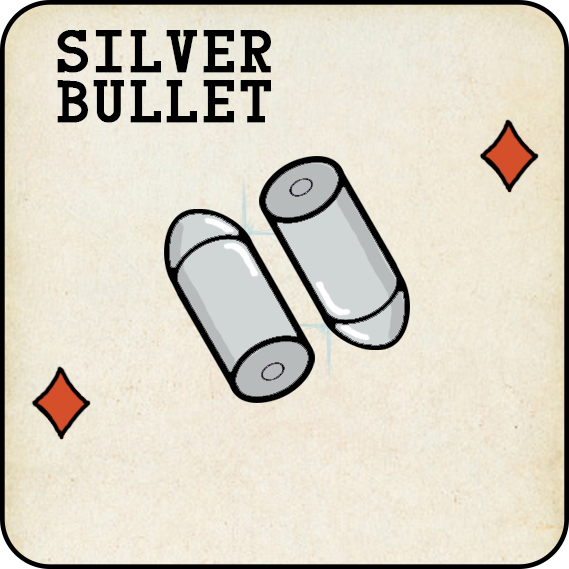
\includegraphics[width=0.5\textwidth]{silverB.png}
    \caption{Beispiel: "Silver Bullet"}
\end{figure}

\begin{figure}[H]
    \centering
    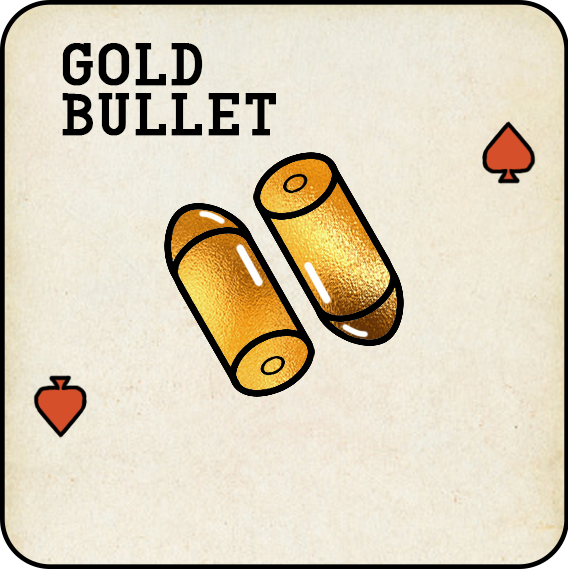
\includegraphics[width=0.5\textwidth]{goldB.png}
    \caption{Beispiel: "Gold Bullet"}
\end{figure}

\begin{figure}[H]
    \centering
    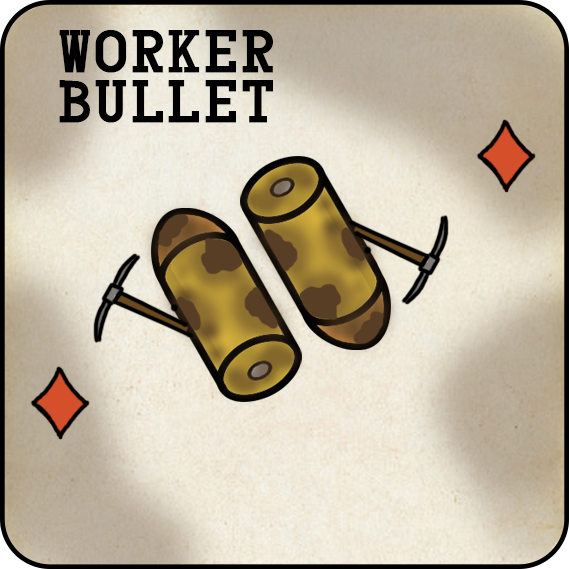
\includegraphics[width=0.5\textwidth]{workerB.png}
    \caption{Beispiel: "Worker Bullet"}
\end{figure}

\begin{figure}[H]
    \centering
    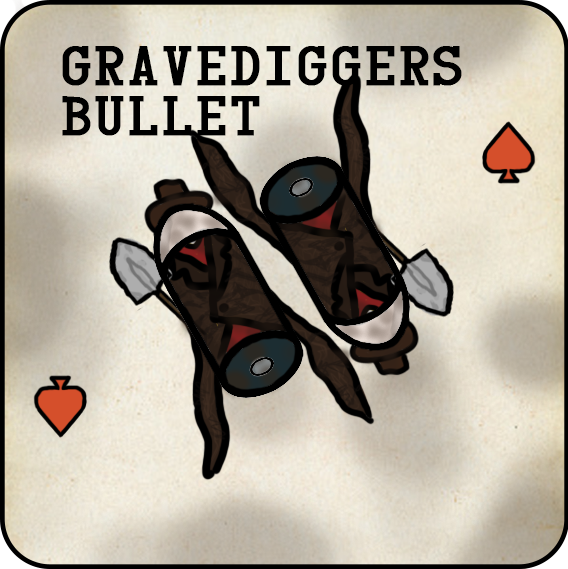
\includegraphics[width=0.5\textwidth]{graveB.png}
    \caption{Beispiel: "GravediggersBullet Bullet"}
\end{figure}


Die zweite Säule: Schutz:
Die Säule des Schutzes beschäftigt sich damit, gegnerische Angriffe abzuwehren. Dazu gehören Bullets, die dem Spieler
Schutz geben oder besonders stark beim Parieren sind. Schutz ist die kleinste und unwichtigste Säule der drei,
da jede Bullet die Möglichkeit bietet, mit ihr zu parieren und damit Schaden abzuwehren. Jedoch sind auch einfach nur große,
starke Bullets wichtig, um hohe Angriffe von Gegnern abzublocken. Da jede Bullet parieren kann, gibt es nicht wirklich Staples,
"Turtle Bullet" ist jedoch die beste Wahl für eine einfache und starke Schutz-Bullet.

\begin{figure}[H]
    \centering
    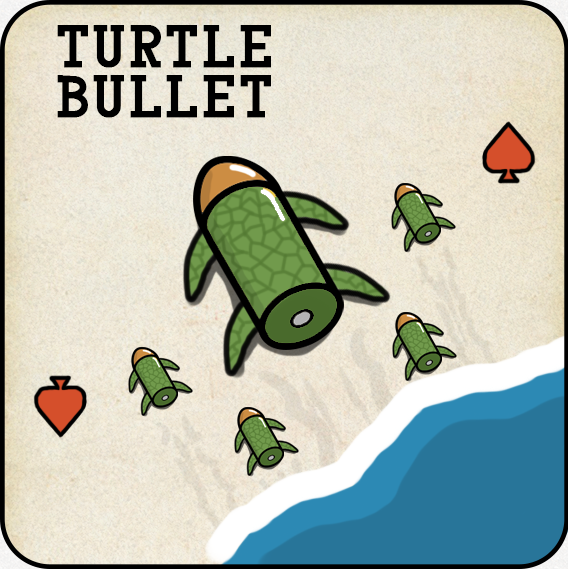
\includegraphics[width=0.5\textwidth]{turtleB.png}
    \caption{Beispiel: "Turtle Bullet"}
\end{figure}

Die dritte Säule: Wincon:
Die dritte Säule ist der Kern eines Decks und beinhaltet alle Karten, die dafür verwendet werden, durch die Deckstrategie einen Kampf zu gewinnen.
Das Wort "Wincon" bezieht sich dabei auf die Wincondition, welche je nach Archetyp des Decks unterschiedlich ist.
Ein Rotation Deck hat andere Karten in der dritten Säule als ein Destroy Deck. Stables existieren nur in den jeweiligen Archetypen
und nicht in der Gesamtheit der Wincon, auch wenn es einzelne Karten gibt, die so stark sind, dass sie in mehreren Decks verwendet werden können.
Ein Beispiel dafür ist "Bull et" oder "Bewitched Bullet".

\begin{figure}[H]
    \centering
    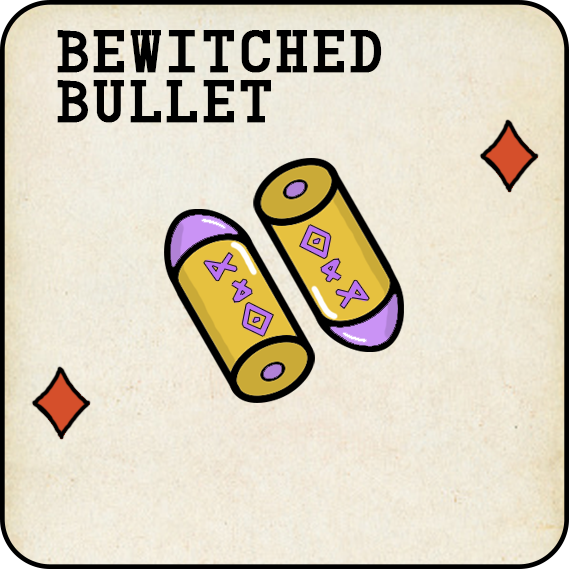
\includegraphics[width=0.5\textwidth]{bewitched_Bullet.png}
    \caption{Beispiel: Bewitched Bullet}
\end{figure}

\begin{figure}[H]
    \centering
    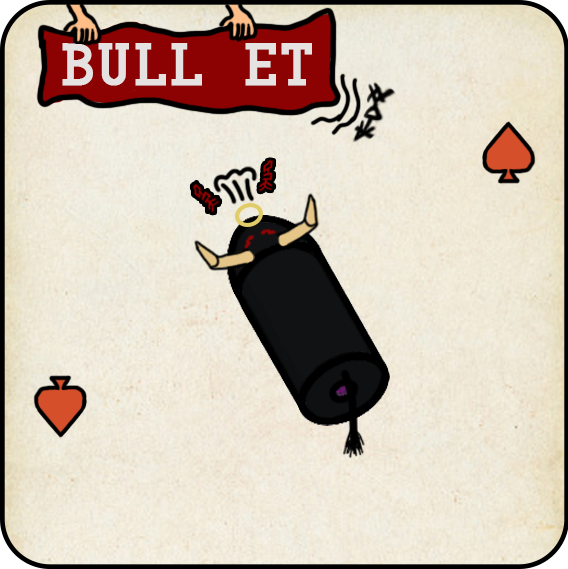
\includegraphics[width=0.5\textwidth]{bull_et.png}
    \caption{Beispiel: Bewitched Bullet}
\end{figure}

\subsection{Encounter modifier? Was steck dahinter?}\label{subsec:placementMatters}

Der Spieler hat die Möglichkeit, mehrere Decks zu bauen und zwischen bis zu fünf Decks hin und her zu wechseln.
Um den Spieler dazu zu bringen, auch mal ein anderes Deck zu spielen und nicht immer das selbe, und um mehr
Abwechslung ins Spiel zu bringen, wurden Encounter Modifier eingeführt.
Diese Modifier ändern die Spielregeln mal leicht, mal schwer und je nachdem haben große Auswirkungen darauf, wie der Spieler das Spiel spielt.
Ein Beispiel für einen Modifier, welcher das Ändern des Decks als Ziel hat, ist "Moist". Durch "Moist" verliert jede Bullet einen Dmg ihrer Dmg-Value,
wenn sie im Revolver rotiert.
Das wirkt sich vor allem auf Decks aus, welche auf Rotationen basieren. Diese Decks sind noch immer spielbar, jedoch geschwächt.
Ein Beispiel für einen Encounter Modifier, welcher mehr Abwechslung ins Spiel bringt, ist "Steel Nerves". "Steel Nerves" führt
einen Timer ein, welcher, falls er Null erreicht, den Revolver automatisch schießt. Das bringt einen gewissen Zeitdruck
ins Spiel und der Spieler muss mit der Stresssituation umgehen und dabei weiterhin versuchen, gute Züge zu spielen, um den Gegner zu besiegen. %TODO Bilder von Encounter Modifier

\subsection{Enemy Gamedesign and difficulty scaling}\label{subsec:placementMatters}

Der Gegner ist ein wichtiger Teil des Gameplays von \FF. Er dient nicht nur als Ziel für die Angriffe des Spielers, ohne ihn gäbe es kein Gameplay.
Der Gegner reagiert nicht auf den Spieler, sondern der Spieler reagiert auf den Gegner. Der Gegner zeigt seine nächste Aktion über seinem Kopf an, noch während der Spieler am Zug ist.
Das bewirkt, dass der Spieler seinen Zug anpasst, je nachdem was der Gegner plant. Jedoch kann der Spieler die Pläne des Gegners auch einfach ignorieren,
falls er gerade andere Spielzüge vorbereitet oder glaubt, dass die Aktion des Gegners ihm keine Probleme bereitet.


Ein Gegner kann verschiedene Aktionen ausführen, dazu zählt Schaden zu verursachen, welcher von dem Spieler pariert
werden kann, sich selbst Schild zu geben oder eine gegnerspezifische Aktion auszuführen. Der Gegnertyp bestimmt,
wie viel Schaden der Gegner macht, wie viel Schild er sich selbst geben kann und welche Aktionen er ausführen kann.
Die Witch zum Beispiel kann den Revolver des Spielers nach links drehen.


Gegnertypen sind in verschiedene Klassen eingeteilt,
was durch ihre Effektivität in verschiedenen Kampfszenarien bestimmt wird. Der Pyro ist ein Support-Gegner, da er vor
allem zusammen mit anderen Gegnern glänzt, da er den Spieler in Brand setzt, damit die anderen Gegner mit ihren Angriffen
mehr Schaden machen. Außerdem sorgt die Aktion "Hot Potato" dafür, dass dem Spieler die Reserven knapp werden. "Hot Potato"
gibt dem Spieler "Scorching Bullet" in die Hand, eine feindliche Bullet, welche dem Spieler zehn Schaden verursacht immer am
Ende eines Zuges, falls sich “Scorching Bullet” in der Hand des Spielers oder im Revolver befindet. Sie kostet drei Reserves,
bekommt der Spieler sie also in die Hand, muss er sich entscheiden, ob er die Bullet behält und seine Reserves für etwas anderes
verwendet oder er die drei Reserves bezahlt und die Bullet damit in den Revolver lädt und wegschießt.


Die Gegner sind so konfiguriert, dass oft Schaden durchgeht, selbst wenn der Spieler etwas pariert. Die Mindestanzahl
an Schaden ist sieben, da die normale Bullet sechs Schaden macht, also die Anfangskarten nicht ausreichen, um den gesamten
Schaden zu parieren. Gegner sind außerdem in Phasen eingeteilt, wobei jede Phase immer mehr Schaden macht als die letzte.
Das wird gemacht, damit der Spieler am Anfang des Kampfes sich ein Spielfeld aufbauen kann, und er weniger Schaden bekommt,
wenn er ein gutes Deck hat und damit den Gegner in wenigen Zügen schon besiegen kann oder sich eine Combo aufbauen kann,
um den erhöhten Schaden irgendwie zu verhindern. Das spielt wiederum mit dem Genre des Rogue-Lites zusammen,
da der Spieler am Anfang des Spiels schlechter sein soll als wenn er schon länger spielt oder schon ein oder zwei Mal gestorben ist.


Gegnertypen sind oft um eine Mechanik konzipiert und dienen oft als Gegenstück zu bestimmten Archetypen oder unterstützen
sogar manchmal Archetypen, wie \zB die Witch, die durch das Linksdrehen des Revolvers dem Rotations-Archetyp hilft.


Kämpfe sind in einer Encounter-Konfigurationsdatei definiert, die basierend auf dem Fortschritt des Spielers passende
Kämpfe aus der Liste auswählt. In dieser Datei werden auch Encounter-Modifiers definiert, damit die Schwierigkeit
der Kämpfe besser kontrolliert werden kann. Außerdem können damit illegale Encounter-Modifier-Kombinationen verhindert
werden, also Kombinationen, die nicht miteinander funktionieren. Je näher der Spieler an der nächsten Area ist,
desto schwieriger werden die Kämpfe. Kämpfe sind so definiert, dass falls ein neuer Gegnertyp das erste Mal vorkommt,
zumindest einmal ein Kampf von dem Spieler absolviert wird, bei dem er nur gegen diesen neuen Gegnertyp kämpft.


Auch wenn an den Gegnern und deren "Difficulty Balancing" seit schon einem jahr gearbeitet wird, gibt es noch immer viele
zu tun und zu verbessern, da das spiel im Moment zu einfach ist.



\subsection{Carddescriptions}\label{subsec:placementMatters}

Wichtig in einem Kartenspiel wie \FF sind die Beschreibungen der Effekte der Karten. Die Terminologie der Beschreibungen
soll konsistent, verständlich und so kurz wie möglich sein, ohne dass Informationen dabei verloren geht. Bei \FF sind
Effekt Trigger Wörter, welche mit Bindestrichen zusammengehängt werden. Sie sind verknüpft mit dem Wort "on" am Phrasen Anfang, um zu symbolisieren,
dass der Effekt "on", also auf diesem Event getriggert wird. Zusätzlich soll der Trigger auch verständlich sein ohne ihn zu erklären.
"On-Placedown" zum Beispiel aktiviert den Effekt, wenn die Bullet in den Revolver gelegt wird, also "down geplaced" wird.
Diese Art von Trigger wird intern "Major Trigger" genannt.


Übergeordnet über den "Major Triggern" sind die "Trigger Conditions". Sie werden zuerst gecheckt, wie zum Beispiel die "While in Revolver:" Condition.
Der nachfolgende "On-Turn-Begin" Trigger kann nur getriggert werden, wenn die Condition erfüllt ist, also wenn die Bullet sich im Revolver befindet. %TODO Bild von workers Bullet Effekt hier


Sogenannte "spezifische Trigger" werden ausgeschrieben, da sie zu lang, zu spezifisch und zu selten für die Schreibweise der "Major Trigger" sind. Ein Beispiel dafür ist
"Whenever this rotates into the slot that it was originally placed into:".


Zusätzlich zu abgekürzten Trigger-Bezeichnungen gibt es Keywords. Keywords in \FF sind Effekte, die immer die gleiche
Erklärung haben und deswegen wird die Erklärung in eine extra Info-Box ausgelagert.
Keywords sind ein guter Weg, erfahrenen Spielern die Infos auf einem Blick zu geben, da sie bereits grob wissen, was das
Keyword bedeutet, trotzdem aber neuen Spielern die Möglichkeit zu bieten, sich die Erklärung noch einmal durchzulesen.
Keywords werden angewendet bei "Trait-Effekten" und "Status-Effekten". Trait-Effekte sind extra Eigenschaften für Bullets
wie zum Beispiel "spray", durch welchen alle Gegner von der Bullet getroffen werden anstatt nur einer.
Um Status-Effekte und Trait-Effekte variabel zu halten, werden Parameter verwendet. %TODO Bild mit Erklärung zu Parametern noch



%keywords -> für flvor und damit der psiler der schon läänger spielt nicht immer alles lesen muss. und statuseffekte---------------------------------------------------------------------------------------------
%Slots und sloticons


%\subsection{Tutoriel}\label{subsec:placementMatters}


%Broad Bullet design für draft

%

%gegner gamedesign :((((

\subsection{Wie eine Entscheidung das Spiel verändert am Beispiel des Kartennachziehens}\label{subsec:placementMatters}

Während der Entwicklung eines Kartenspieles müssen viele Entscheidungen getroffen werden, wie \zB die Entscheidung,
Karten, welche geschossen wurden nun wieder unter das Deck zu legen. In früheren \FF Versionen wurden geschossene Karten einfach aus dem Kampf entfernt.
Jedoch waren die Kämpfe dadurch relativ schnell vorbei für den Spieler, da nur mehr normale Bullets gezogen wurden nachdem das Deck leer gezogen wurde.
Dadurch das das Deck nach der Änderung nie leer wird, bleibt der Kampf interessant.
Das Spiel wurde auf einen Schlag viel dynamischer und es konnten viel mehr verschiedene und stärkere Combos ausgeführt werden. Das "Cyclen"
von Karten ist wichtig, da Karten dadurch in einem Kampf öfters verwendet werden können. Decks sind abwechslungsreicher und das Potenzial der Bullets
kann besser von dem Spieler benutzt werden.


Diese simple Änderung zeigt, dass auch nur die kleinste Entscheidung das Spiel komplett verändern kann, weshalb Playtesting
wichtig für ein Spiel wie \FF ist. Dies wurde auch bei der technischen Umsetzung bedacht, weshalb \FF über so viele Configfiles verfügt.


\subsection{Gameplay-Reworks}\label{subsec:placementMatters}
Über die Entwicklung von \FF gab es viele verschiedene Versionen, manche mit kleinen Änderungen, manche jedoch mit komplett veränderten Mechaniken und Regeln.
Die Entwicklung der jetzigen Version zog sich über 2 Jahre.


Unter anderem wurde das damalige Schutzsystem der Cover-Karten mit dem jetzigen Parry-System ausgetauscht.
Cover-Karten waren ein zusätzlicher Kartentyp zu den Bullets, hinter welchen sich der Spieler "verstecken" konnte.
Bei Tests gab es jedoch einige Probleme mit den Covern, da sich die Spieler immer nur hinter den Covern versteckten
und dadurch eine pasive spielweiße unterstütz wurde. Um diesem Problem entgegenzuwirken, wurde die Parry-Mechanik eingeführt,
welche auch Bullets zum Schutz des Spielers verwendet, um sich mehr auf den Kern von \FF - die Bullets - zu konzentrieren.
Das Einführen von Parry markiert den Start der jetzigen \FF Version.

% resets author
\renewcommand{\kapitelautor}{}
